\documentclass[12pt,a4paper]{article}

%%%%%%%%%%%%%%%%%%%%%%%%%%%%%%%%%%%%%%%%%%%%%%%%%%%%%%%%%%%%%%%%%%%%%%%%%
%
%   LaTeX File for Doctor (Master) Thesis of Tsinghua University
%   LaTeX + CJK     清华大学博士(硕士)论文模板
%   Based on Wang Tianshu's Template for XJTU
%	Version: 1.00
%   Last Update: 2003-09-12
%
%%%%%%%%%%%%%%%%%%%%%%%%%%%%%%%%%%%%%%%%%%%%%%%%%%%%%%%%%%%%%%%%%%%%%%%%%
%   Copyright 2002-2003  by  Lei Wang (BaconChina)       (bcpub@sina.com)
%%%%%%%%%%%%%%%%%%%%%%%%%%%%%%%%%%%%%%%%%%%%%%%%%%%%%%%%%%%%%%%%%%%%%%%%%

%%%%%%%%%%%%%%%%%%%%%%%%%%%%%%%%%%%%%%%%%%%%%%%%%%%%%%%%%%%%%%%%%%%%%%%%%
%
%   LaTeX File for phd thesis of xi'an Jiao Tong University
%
%%%%%%%%%%%%%%%%%%%%%%%%%%%%%%%%%%%%%%%%%%%%%%%%%%%%%%%%%%%%%%%%%%%%%%%%%
%   Copyright 2002  by  Wang Tianshu    (tswang@asia.com)
%%%%%%%%%%%%%%%%%%%%%%%%%%%%%%%%%%%%%%%%%%%%%%%%%%%%%%%%%%%%%%%%%%%%%%%%%

%%%%%%%%%%%%%%%%%%%%%%%%%%%%%%%%%%%%%%%%%%%%%%%%%%%%%%%%%%%
%
% 引用的宏包和相应的定义
%
%%%%%%%%%%%%%%%%%%%%%%%%%%%%%%%%%%%%%%%%%%%%%%%%%%%%%%%%%%%

\usepackage[dvips]{graphicx}
\usepackage{subfigure}
% 支持彩色
\usepackage{color}
% eps图像
\usepackage{epsfig}

%\else
%\usepackage[dvips]{graphicx}
%\usepackage{subfigure}
%\fi

% 首行缩进宏包
\usepackage{indentfirst}

% 版面控制宏包,定义规定的版面尺寸
\usepackage[%top=2cm,
            %body={14.6true cm,22true cm},
            twosideshift=0 pt,
            %headheight=1.0true cm
		top=1in,bottom=1.5in,left=1.25in,right=1.25in
            ]{geometry}

% 脚注控制
\usepackage[perpage,symbol]{footmisc}

% AMSLaTeX宏包 用来排出更加漂亮的公式
\usepackage{amsmath}
\usepackage{amssymb}

% 不同于\mathcal or \mathfrak 之类的英文花体字体
\usepackage{mathrsfs}

% 定理类环境宏包,其中 amsmath 选项用来兼容 AMS LaTeX 的宏包
\usepackage[amsmath,thmmarks]{ntheorem}

% 因为图形可浮动到当前页的顶部,所以它可能会出现
% 在它所在文本的前面. 要防止这种情况,可使用 flafter
% 宏包
%\usepackage{flafter}

%浮动图形控制宏包
%允许上一个section的浮动图形出现在下一个section的开始部分
%该宏包提供处理浮动对象的 \FloatBarrier 命令,使所有未处
%理的浮动图形立即被处理
\usepackage[below]{placeins}

% 图文混排用宏包
%\usepackage{floatflt}

% 图形和表格的控制
\usepackage{rotating}

% tex1cm宏包,控制字体的大小
\usepackage{type1cm}

% 控制标题的宏包
\usepackage[sf]{titlesec}

% 控制目录的宏包
\usepackage{titletoc}

% 处理数学公式中的黑斜体的宏包
\usepackage{bm}

%可将浮动对象放置到文件的最后
%\usepackage{endfloat}

% fancyhdr宏包 页眉和页脚的相关定义
\usepackage{fancyhdr}
\usepackage{fancyref}

% 支持引用的宏包
\usepackage{cite}

%浮动图形和表格标题样式
\usepackage{caption2}

% 定制表格和图形的多行标题行距
\usepackage{setspace}

% 打印当前页面格式的宏包
\usepackage{layouts}

% 使用Times字体的宏包
%\usepackage{times}

% qiuying add
\usepackage[CJKtextspaces]{xeCJK}
\usepackage{tikz}

% 生成带书签的pdf
\usepackage[dvipdfmx,
            CJKbookmarks=true,
            bookmarksnumbered=true,
            bookmarksopen=true,
            pdfborder=001,
            citecolor=blue,
            anchorcolor=green,
            urlcolor=blue,
	  pdfcreator={XeTeX,XeCJK},
	  pdfproducer={XeTeX},% 这个好像没起作用? 
	  pdftitle={四位无线链路估计},
	  pdfsubject={4bitle},
	  pdfauthor={qiuying},
	  pdfkeywords={4bitle},
	  %pdfpagemode={FullScreen},
	  colorlinks={true},
	  linkcolor={blue} %改变目录、引用的颜色
            ]{hyperref}


\title{\textsf{四位无线链路估计}}
\author{
\textit{\small Rodrigo Fonseca, Omprakash Gnawali, Kyle Jamieson, Philip Levis}\\
{\kai 译\song :\kai 裘莹}}
\date{}

%%%%%%%%%%%%%%%%%%%%%%%%%%%%%%%%%%%%%%%%%%%%%%%%%%%%%%%%%%%%%%%%%%%%%%%%%
%
%   LaTeX File for Doctor (Master) Thesis of Tsinghua University
%   LaTeX + CJK     清华大学博士(硕士)论文模板
%   Based on Wang Tianshu's Template for XJTU
%   Version: 1.00
%   Last Update: 2003-09-12
%
%%%%%%%%%%%%%%%%%%%%%%%%%%%%%%%%%%%%%%%%%%%%%%%%%%%%%%%%%%%%%%%%%%%%%%%%%
%   Copyright 2002-2003  by  Lei Wang (BaconChina)       (bcpub@sina.com)
%%%%%%%%%%%%%%%%%%%%%%%%%%%%%%%%%%%%%%%%%%%%%%%%%%%%%%%%%%%%%%%%%%%%%%%%%

%%%%%%%%%%%%%%%%%%%%%%%%%%%%%%%%%%%%%%%%%%%%%%%%%%%%%%%%%%%%%%%%%%%%%%%%%
%
%   LaTeX File for phd thesis of xi'an Jiao Tong University
%
%%%%%%%%%%%%%%%%%%%%%%%%%%%%%%%%%%%%%%%%%%%%%%%%%%%%%%%%%%%%%%%%%%%%%%%%%
%   Copyright 2002  by  Wang Tianshu    (tswang@asia.com)
%%%%%%%%%%%%%%%%%%%%%%%%%%%%%%%%%%%%%%%%%%%%%%%%%%%%%%%%%%%%%%%%%%%%%%%%%
%%%%%%%%%%%%%%%%%%%%%%%%%%%%%%%%%%%%%%%%%%%%%%%%%%%%%%%%%%%
%
% 主文档 格式定义
%
%%%%%%%%%%%%%%%%%%%%%%%%%%%%%%%%%%%%%%%%%%%%%%%%%%%%%%%%%%%

% 按清华标准, 将版芯控制在240mm以内, 正文范围控制在220mm以内
%\addtolength{\headsep}{-0.1cm}          %页眉位置
%\addtolength{\footskip}{-0.1cm}         %页脚位置
\addtolength{\topmargin}{0.5cm}

%%%%%%%%%%%%%%%%%%%%%%%%%%%%%%%%%%%%%%%%%%%%%%%%%%%%%%%%%%%
% 公式的精调
%%%%%%%%%%%%%%%%%%%%%%%%%%%%%%%%%%%%%%%%%%%%%%%%%%%%%%%%%%%

%\setlength{\mathindent}{4.7 em}     %左对齐公式缩进量

% \eqnarray如果很长,影响分栏、换行和分页(整块挪动,造成页面空白),
% 可以设置成为自动调整模式
\allowdisplaybreaks[4]

%%%%%%%%%%%%%%%%%%%%%%%%%%%%%%%%%%%%%%%%%%%%%%%%%%%%%%%%%%%
%下面这组命令使浮动对象的缺省值稍微宽松一点,从而防止幅度
%对象占据过多的文本页面,也可以防止在很大空白的浮动页上放置
%很小的图形。
%%%%%%%%%%%%%%%%%%%%%%%%%%%%%%%%%%%%%%%%%%%%%%%%%%%%%%%%%%%
\renewcommand{\textfraction}{0.15}
\renewcommand{\topfraction}{0.85}
\renewcommand{\bottomfraction}{0.65}
\renewcommand{\floatpagefraction}{0.60}


%%%%%%%%%%%%%%%%%%%%%%%%%%%%%%%%%%%%%%%%%%%%%%%%%%%%%%%%%%%
%下面这组命令可以使公式编号随着每开始新的一节而重新开始。
%%%%%%%%%%%%%%%%%%%%%%%%%%%%%%%%%%%%%%%%%%%%%%%%%%%%%%%%%%%

%\makeatletter      % '@' is now a normail "letter" for TeX
%\@addtoreset{eqation}{section}
%\makeatother       % '@' is restored as a "non-letter" character for TeX

%%%%%%%%%%%%%%%%%%%%%%%%%%%%%%%%%%%%%%%%%%%%%%%%%%%%%%%%%%%
% 重定义字体命令
%%%%%%%%%%%%%%%%%%%%%%%%%%%%%%%%%%%%%%%%%%%%%%%%%%%%%%%%%%%
% 注意win2000,没有 simsun, 最好到网上找一个
% 一些字体是office2000 带的
%%%%%%%%%%%%%%%%%%%%%%%%%%%%%%%%%%%%%%%%%%%%%%%%%%%%%%%%%%%

\setmainfont{TeX Gyre Termes}
\setsansfont{TeX Gyre Heros}
\setmonofont{TeX Gyre Cursor}
%\setCJKmainfont[BoldFont={方正小标宋简体}]{Adobe Song Std}    % 宋体
%\setCJKsansfont{Adobe Heiti Std}
%\setCJKmonofont{Adobe Fangsong Std}
\setCJKmainfont{SimSun}    % 宋体
\setCJKsansfont{SimHei}
\setCJKmonofont{FangSong_GB2312}

%\setCJKfamilyfont{song}[BoldFont={方正宋黑简体}]{SimSun}      	% 宋体
%\setCJKfamilyfont{song}[BoldFont={方正宋三_GBK}]{方正博雅宋_GBK}  % 宋体
%\setCJKfamilyfont{song}[BoldFont={Adobe Heiti Std}]{Adobe Song Std}    % 宋体
%\setCJKfamilyfont{song}[BoldFont={华文中宋}]{华文宋体}    % 宋体
%\setCJKfamilyfont{song}[BoldFont={方正大标宋_GBK}]{方正兰亭宋_GBK}    % 宋体
%\setCJKfamilyfont{song}[BoldFont={方正小标宋简体}]{方正书宋简体}    % 宋体
%文泉驿微米黑
%\setCJKfamilyfont{song}[BoldFont={方正小标宋简体}]{Adobe Song Std}    % 宋体
\setCJKfamilyfont{song}{SimSun}    			% 宋体
\setCJKfamilyfont{hei}{SimHei}      		% 黑体
\setCJKfamilyfont{kai}{KaiTi_GB2312}      	% 楷体
\setCJKfamilyfont{fang}{Fangsong_GB2312}  	% 仿宋体
\setCJKfamilyfont{nwpulogo}{nwpulogo}     	% 含"西北工业大学"logo字体

\newcommand{\song}{\CJKfamily{song}}
\newcommand{\hei}{\CJKfamily{hei}}
\newcommand{\fang}{\CJKfamily{fang}}
\newcommand{\kai}{\CJKfamily{kai}}
\newcommand{\nwpulogo}{\CJKfamily{nwpulogo}}

%%%%%%%%%%%%%%%%%%%%%%%%%%%%%%%%%%%%%%%%%%%%%%%%%%%%%%%%%%%
% 重定义字号命令
%%%%%%%%%%%%%%%%%%%%%%%%%%%%%%%%%%%%%%%%%%%%%%%%%%%%%%%%%%%

\newcommand{\chuhao}{\fontsize{42pt}{63pt}\selectfont}    % 初号, 1.5倍行距
\newcommand{\yihao}{\fontsize{26pt}{36pt}\selectfont}    % 一号, 1.4倍行距
\newcommand{\erhao}{\fontsize{22pt}{28pt}\selectfont}    % 二号, 1.25倍行距
\newcommand{\xiaoer}{\fontsize{18pt}{18pt}\selectfont}    % 小二, 单倍行距
\newcommand{\sanhao}{\fontsize{16pt}{24pt}\selectfont}    % 三号, 1.5倍行距
\newcommand{\xiaosan}{\fontsize{15pt}{22pt}\selectfont}    % 小三, 1.5倍行距
\newcommand{\sihao}{\fontsize{14pt}{21pt}\selectfont}    % 四号, 1.5倍行距
\newcommand{\banxiaosi}{\fontsize{13pt}{16.25pt}\selectfont}    % 半小四, 1.25倍行距
\newcommand{\xiaosi}{\fontsize{12.5pt}{12.5pt}\selectfont}    % 小四, 1.2倍行距
\newcommand{\dawuhao}{\fontsize{11pt}{11pt}\selectfont}    % 大五号, 单倍行距
\newcommand{\wuhao}{\fontsize{10.5pt}{10.5pt}\selectfont}    % 五号, 单倍行距
\newcommand{\xiaowu}{\fontsize{9pt}{9pt}\selectfont}		% 小五号



%%%%%%%%%%%%%%%%%%%%%%%%%%%%%%%%%%%%%%%%%%%%%%%%%%%%%%%%%%%
% 重定义一些正文相关标题
%%%%%%%%%%%%%%%%%%%%%%%%%%%%%%%%%%%%%%%%%%%%%%%%%%%%%%%%%%%

% qiuying comment
%\theoremstyle{plain} \theorembodyfont{\song\rmfamily}
%\theoremheaderfont{\hei\rmfamily} \theoremseparator{:}
%\newtheorem{definition}{\hei 定义}[chapter]
%\newtheorem{proposition}[definition]{\hei 命题}
%\newtheorem{lemma}[definition]{\hei 引理}
%\newtheorem{theorem}{\hei 定理}[chapter]
%\newtheorem{axiom}{\hei 公理}
%\newtheorem{corollary}[definition]{\hei 推论}
%\newtheorem{exercise}[definition]{}
%
%\theoremheaderfont{\CJKfamily{hei}\rmfamily}\theorembodyfont{\rmfamily}
%\theoremstyle{nonumberplain} \theoremseparator{:}
%\theoremsymbol{$\blacksquare$}
%\newtheorem{proof}{\hei 证明}
%
%\theoremsymbol{$\square$}
%\newtheorem{example}{\hei 例}
%

%%%%%%%%%%%%%%%%%%%%%%%%%%%%%%%%%%%%%%%%%%%%%%%%%%%%%%%%%%%
% 用于中文段落缩进 和正文版式
%%%%%%%%%%%%%%%%%%%%%%%%%%%%%%%%%%%%%%%%%%%%%%%%%%%%%%%%%%%
%\CJKcaption{GB_aloft}
\xeCJKcaption{gb_452}

\newlength \CJKtwospaces

\def\CJKindent{
    \settowidth\CJKtwospaces{\CJKchar{"0A1}{"0A1}\CJKchar{"0A1}{"0A1}}%
    \parindent\CJKtwospaces
}


%\CJKtilde  \CJKindent

\renewcommand\contentsname{目~~~~录}
\renewcommand\chaptername{\CJKprechaptername\CJKthechapter\CJKchaptername}

%%%%%%%%%%%%%%%%%%%%%%%%%%%%%%%%%%%%%%%%%%%%%%%%%%
%定义段落章节的标题和目录项的格式
%%%%%%%%%%%%%%%%%%%%%%%%%%%%%%%%%%%%%%%%%%%%%%%%%%
\setcounter{secnumdepth}{4}
\setcounter{tocdepth}{2}

% Modified By Lei Wang BaconChina
% THU Version
\titleformat{\chapter}[hang]
    {\normalfont\sanhao\filcenter\hei\sf}
    {\sanhao{\chaptertitlename}}
    {20pt}{\sanhao}
%\titlespacing{\chapter}{0pt}{-3ex  plus .1ex minus .2ex}{2.5ex plus .1ex minus .2ex}
\titlespacing{\chapter}{0pt}{-3ex  plus .1ex minus .2ex}{0.25em}

\titleformat{\section}[hang]{\hei \sf \sihao}
    {\sihao \thesection}{0.5em}{}{}
%\titlespacing{\section}{0pt}{1.5ex plus .1ex minus .2ex}{\wordsep}
\titlespacing{\section}{0pt}{0.5em}{0em}

\titleformat{\subsection}[hang]{\hei \sf \banxiaosi}
    {\banxiaosi \thesubsection}{0.5em}{}{}
%    {\banxiaosi \thesubsection}{0pt}{}{}
%\titlespacing{\subsection}{0pt}{1.5ex plus .1ex minus .2ex}{\wordsep}
\titlespacing{\subsection}{0pt}{0.25em}{0em}

\titleformat{\subsubsection}[hang]{\hei \sf}
    {\thesubsubsection }{0.5em}{}{}
%\titlespacing{\subsubsection}{0pt}{1.2ex plus .1ex minus .2ex}{\wordsep}
\titlespacing{\subsubsection}{0pt}{0.25em}{0pt}

%去掉中间对齐的sectionformat,这样就把节的标题左对齐了。
%\renewcommand \sectionformat{}

% 按清华标准, 缩小目录中各级标题之间的缩进
\dottedcontents{chapter}[0.0em]{\hei\vspace{0.5em}}{0.0em}{5pt}
\dottedcontents{section}[1.16cm]{}{1.8em}{5pt}
\dottedcontents{subsection}[2.00cm]{}{2.7em}{5pt}
\dottedcontents{subsubsection}[2.86cm]{}{3.4em}{5pt}

%%%%%%%%%%%%%%%%%%%%%%%%%%%%%%%%%%%%%%%%%%%%%%%%%%%%%%%
% 定义页眉和页脚 使用fancyhdr 宏包
%%%%%%%%%%%%%%%%%%%%%%%%%%%%%%%%%%%%%%%%%%%%%%%%%%%%%%%%

\newcommand{\makeheadrule}{%
    \makebox[0pt][l]{\rule[.7\baselineskip]{\headwidth}{0.8pt}}%
% 1 Line Modified by Lei Wang BaconChina
% XJTU Version
%    \rule[.6\baselineskip]{\headwidth}{0.4pt}\vskip-.8\baselineskip}
% THU Version
    \vskip-.8\baselineskip}

\makeatletter
\renewcommand{\headrule}{%
    {\if@fancyplain\let\headrulewidth\plainheadrulewidth\fi
     \makeheadrule}}

\pagestyle{fancyplain}

%去掉章节标题中的数字
\renewcommand{\chaptermark}[1]{\markboth{\chaptername \ #1}{}}

 \fancyhf{}
% \fancyfoot[C,C]{\thepage}

%在book文件类别下,\leftmark自动存录各章之章名,\rightmark记录节标题

% Modified by Lei Wang BaconChina
% XJTU Version
% \fancyhead[RO]{\CJKfamily{song}\leftmark}
% \fancyhead[LE]{\CJKfamily{song}西安交通大学博士学位论文}
% \fancyfoot[C,C]{--~\thepage~--}
% THU Version
% \fancyhead[CO]{\CJKfamily{song}\wuhao\leftmark}
% \fancyhead[CE]{\nwpulogo\fontsize{8pt}{6pt} 西北工业大学~~~ \sanhao\song 本科毕业设计论文}
 \fancyfoot[C,C]{\wuhao \thepage}
\chead{\sanhao\raisebox{0.04cm}{\nwpulogo 西北工业大学} \song \bfseries{本科毕业设计论文}}

%%%%%%%%%%%%%%%%%%%%%%%%%%%%%%%%%%%%%%%%%%%%%%%%%%%%%%%%
% 设置行距和段落间垂直距离
%%%%%%%%%%%%%%%%%%%%%%%%%%%%%%%%%%%%%%%%%%%%%%%%%%%%%%%%

% 段落之间的竖直距离
\setlength{\parskip}{3pt plus1pt minus1pt}

% 定义行距
\renewcommand{\baselinestretch}{1.25}

%%%%%%%%%%%%%%%%%%%%%%%%%%%%%%%%%%%%%%%%%%%%%%%%%%%%%%%%
% 调整列表环境的垂直间距
%%%%%%%%%%%%%%%%%%%%%%%%%%%%%%%%%%%%%%%%%%%%%%%%%%%%%%%%
\let\orig@Itemize =\itemize
\let\orig@Enumerate =\enumerate
\let\orig@Description =\description

\def\Myspacing{\itemsep=5pt \topsep=0pt \partopsep=0pt \parskip=0pt \parsep=0pt}

\def\newitemsep{
\renewenvironment{itemize}{\orig@Itemize\Myspacing}{\endlist}
\renewenvironment{enumerate}{\orig@Enumerate\Myspacing}{\endlist}
\renewenvironment{description}{\orig@Description\Myspacing}{\endlist}
}

\def\olditemsep{
\renewenvironment{itemize}{\orig@Itemize}{\endlist}
\renewenvironment{enumerate}{\orig@Enumerate}{\endlist}
\renewenvironment{description}{\orig@Description}{\endlist}
}

\newitemsep

%%%%%%%%%%%%%%%%%%%%%%%%%%%%%%%%%%%%%%%%%%%%%%%%%%%%%%%
% 修改引用的格式,
%%%%%%%%%%%%%%%%%%%%%%%%%%%%%%%%%%%%%%%%%%%%%%%%%%%%%%%

%第一行在引用处数字两边加方框
%第二行去除参考文献里数字两边的方框
%\makeatletter
%\def\@cite#1{\mbox{$\m@th^{\hbox{\@ove@rcfont[#1]}}$}}
%\renewcommand\@biblabel[1]{#1}
%\makeatother

% 增加 \ucite 命令使显示的引用为上标形式
\newcommand{\ucite}[1]{$^{\mbox{\scriptsize \cite{#1}}}$}

%%%%%%%%%%%%%%%%%%%%%%%%%%%%%%%%%%%%%%%%%%%%%%%%%%%%%%%%%%%
%
% 定制浮动图形和表格标题样式
%
%%%%%%%%%%%%%%%%%%%%%%%%%%%%%%%%%%%%%%%%%%%%%%%%%%%%%%%%%%%

% \renewcommand{\captionfont}{\CJKfamily{song}\rmfamily}
% \renewcommand{\captionlabelfont}{\CJKfamily{song}\rmfamily}
%
% % 按清华标准, 去掉图表号后面的:
% \renewcommand{\captionlabeldelim}{\hspace{1em}}
%
% % 按清华标准, 图表标题字体为11pt, 这里写作大五号
% \renewcommand{\captionfont}{\wuhao}

%%%%%%%%%%%%%%%%%%%%%%%%%%%%%%%%%%%%%%%%%%%%%%%%%%%%%%%
% 定义题头格言的格式
%%%%%%%%%%%%%%%%%%%%%%%%%%%%%%%%%%%%%%%%%%%%%%%%%%%%%%%

%
% 用法 \begin{Aphorism}{author}
%         aphorism
%      \end{Aphorism}

\newsavebox{\AphorismAuthor}
\newenvironment{Aphorism}[1]
{\vspace{0.5cm}\begin{sloppypar} \slshape
\sbox{\AphorismAuthor}{#1}
\begin{quote}\small\itshape }
{\\ \hspace*{\fill}------\hspace{0.2cm} \usebox{\AphorismAuthor}
\end{quote}
\end{sloppypar}\vspace{0.5cm}}

%自定义一个空命令,用于注释掉文本中不需要的部分。
\newcommand{\comment}[1]{}

% This is the flag for longer version
\newcommand{\longer}[2]{#1}

\newcommand{\ds}{\displaystyle}

% define graph scale
\def\gs{1.0}

%%%%%%%%%%%%%%%%%%%%%%%%%%%%%%%%%%%%%%%%%%%%%%%%%%%%%%%%%%%%%%%%%%%%%%
% 自定义项目列表标签及格式 \begin{denselist} 列表项 \end{denselist}
%%%%%%%%%%%%%%%%%%%%%%%%%%%%%%%%%%%%%%%%%%%%%%%%%%%%%%%%%%%%%%%%%%%%%%
\newcounter{newlist} %自定义新计数器
\newenvironment{denselist}[1][可改变的列表题目]{%%%%%定义新环境
\begin{list}{\textbf{\hei #1} \arabic{newlist}:} %%标签格式
    {
    \usecounter{newlist}
     \setlength{\labelwidth}{22pt} %标签盒子宽度
     \setlength{\labelsep}{0cm} %标签与列表文本距离
     \setlength{\leftmargin}{0cm} %左右边界
     \setlength{\rightmargin}{0cm}
     \setlength{\parsep}{0ex} %段落间距
     \setlength{\itemsep}{0ex} %标签间距
     \setlength{\itemindent}{44pt} %标签缩进量
     \setlength{\listparindent}{22pt} %段落缩进量
    }}
{\end{list}}%%%%%

%添加一些有用的命令
%Chinese style for the chapter reference. It doesn't work with hyperref
\newcommand{\chref}[1]{\CJKnumber{\ref{#1}}}
%adjust Chinese parenthesis space
\newcommand{\KH}[1]{\!\!(#1)\!\!}
\newcommand\dlmu@underline[2][5cm]{\hskip1pt\underline{\hb@xt@ #1{\hss#2\hss}}\hskip3pt}
\let\coverunderline\dlmu@underline

\setlength{\parindent}{2em}
\renewcommand{\lstlistingname}{\wuhao 源码}

\setlength{\headheight}{24pt}

\newfontfamily\codefont{TeX Gyre Cursor}
\newfontfamily\pagella{TeX Gyre Pagella}

\lstdefinelanguage{nesc}
  {morekeywords={components, configuration, event, generic, implementation, includes, interface, module,new, norace, post, provides, signal, task, uses,nx\_struct, nx\_union,command,uint16\_t,uint8\_t,uint32\_t,as,void},sensitive=false,morecomment=[l]{//},morecomment=[s]{/*}{*/},morestring=[b]",}

%\lstset{basicstyle=\codefont\footnotesize,keywordstyle=\color{blue},commentstyle=\color{green},stringstyle=\color{red},tabsize=4,frameround=ffff,escapeinside=``,lineskip=1pt,framerule=0.5pt,xleftmargin=20pt,xrightmargin=10pt,language=nesc,frame=tb,captionpos=b,abovecaptionskip=10pt,numbers=left, framexleftmargin=5mm}
%\lstset{basicstyle=\droidmono\footnotesize,tabsize=4,frameround=ffff,escapeinside=``,lineskip=1pt,framerule=0.5pt,xleftmargin=20pt,xrightmargin=10pt,language=nesc,frame=tb,captionpos=b,abovecaptionskip=10pt,numbers=left, framexleftmargin=5mm}

\definecolor{dkgreen}{rgb}{0,0.6,0}
\definecolor{gray}{rgb}{0.5,0.5,0.5}
\definecolor{mauve}{rgb}{0.58,0,0.82}

\lstset{frame=tb,
  language=Python,
  aboveskip=3mm,
  belowskip=3mm,
  showstringspaces=false,
  columns=flexible,
  basicstyle={\small\ttfamily},
  numbers=none,
  numberstyle=\tiny\color{gray},
  keywordstyle=\color{blue},
  commentstyle=\color{dkgreen},
  stringstyle=\color{mauve},
  breaklines=true,
  breakatwhitespace=true,
  tabsize=4
}

\renewcommand\arraystretch{1.25}


\begin{document}
\sloppy

%%%%%%%%%%%%%%%%%%%%%%%%%%%%%%%%%%%%%%%%%%%%%%%%%%%%%%%%%%%%%%%%%%%%%%%%%
%
%   LaTeX File for Doctor (Master) Thesis of Tsinghua University
%   LaTeX + CJK     清华大学博士(硕士)论文模板
%   Based on Wang Tianshu's Template for XJTU
%   Version: 1.00
%   Last Update: 2003-09-12
%
%%%%%%%%%%%%%%%%%%%%%%%%%%%%%%%%%%%%%%%%%%%%%%%%%%%%%%%%%%%%%%%%%%%%%%%%%
%   Copyright 2002-2003  by  Lei Wang (BaconChina)       (bcpub@sina.com)
%%%%%%%%%%%%%%%%%%%%%%%%%%%%%%%%%%%%%%%%%%%%%%%%%%%%%%%%%%%%%%%%%%%%%%%%%

%%%%%%%%%%%%%%%%%%%%%%%%%%%%%%%%%%%%
% 封一
%%%%%%%%%%%%%%%%%%%%%%%%%%%%%%%%%%%%

\begin{titlepage}
\voffset 2.7cm
\begin{center}
\begin{center}
\begin{minipage}[c]{2.64cm}
\centering
\resizebox{!}{0.9cm}{%
\parbox{0.54cm}{\begin{tikzpicture}
  \draw[line width=0.1cm] (0,0) circle (2cm);
  \draw[line width=0.05cm] (0,0) circle (1.3cm);
  \fill[gray!15] (0,0) circle (1.3cm);
  \fill[white] (0,0) circle (0.9cm);
  \draw[line width=0.05cm] (0,0) circle (0.9cm);
  \fill[black] (-0.5,-0.73) .. controls (-0.35,-0.81) ..
	(-0.2,-0.8)  .. controls (0.15, -0.7) and (0.20,-0.60) .. 
	(0.35,-0.35)   .. controls (0.42, -0.24) and (0.6,-0.26) ..
	(0.6,-0.4)   .. controls (0.58,-0.50) and (0.49, -0.50) ..
	(0.45,-0.45) .. controls (0.4,-0.68) and (0.75, -0.7) ..
	(0.9,0) arc (360:250:0.9cm);
  \fill (-0.4,-0.4)--(-1.33,-0.4)--(1,1.1)--cycle;
  \fill (-0.37,-0.43)--(-0.2,-0.8)--(1.01,1.05)--cycle;
  
  \foreach \x/\txt in {0/N,1/O,2/R,3/T,4/H,5/W,6/E,7/S,8/T,9/E,10/R,11/N,12/~,13/P,14/O,15/L,16/Y,17/T,18/E,19/C,20/H,21/N,22/I,23/C,24/A,25/L,26/~,27/U,28/N,29/I,30/V,31/E,32/R,33/S,34/I,35/T,36/Y}
  {
    \node[scale=0.7,rotate=\x*-6.5-245] at (207+\x*-6.5:1.6cm) {\txt};
  };
  \foreach \x/\txt in {0/西,1/北,2/工,3/业,4/大,5/学}
  {
    \node[scale=1.25,rotate=\x*18-50] at (225+\x*18:1.65cm) {\nwpulogo\txt};
  };
  \foreach \x/\txt in {0/1,1/9,2/3,3/8}
  {
    \node[scale=1,rotate=\x*18-25] at (\x*18-115:1.1cm) {\bfseries\txt};
  };

\end{tikzpicture}
}
}
\end{minipage}
\hskip 0.8cm
\begin{minipage}[c]{8cm}
\fontsize{33}{33}\nwpulogo 西北工业大学
\end{minipage}
\end{center}
\vskip 0.7cm
\chuhao\song {\bfseries 本科毕业设计论文}
\vskip 5cm
{
\sanhao\hei 题~~目 \hspace{0.2cm}\coverunderline[12.5cm]{基于强化学习的轮式机器人决策算法研究}
}
\vskip 2cm
{
\sihao\song 专业名称\coverunderline[7cm]{软件工程}
\vskip 0.7cm
\sihao\song 学生姓名\coverunderline[7cm]{韩~~萧~~阳}
\vskip 0.7cm
\sihao\song 指导教师\coverunderline[7cm]{史~~豪~~斌}
\vskip 0.7cm
\sihao\song 毕业时间\coverunderline[7cm]{2019.07}
\vfill
}
\end{center}
\end{titlepage}

\song \normalsize

\newpage
\maketitle

\xiaosi\song

\begin{abstract}
  我们考虑ad-hoc无线网络中的链路质量估计问题。我们认为要作好链路质量估计必须综合网络层、链路层和物理层的信息。我们为各层设计了窄的、精确的、与协议无关的链路估计接口,它总共提供4位信息:物理层1位,链路层1位,网络层2位。在我们大规模的多跳测试中,使用了这些接口的设计和实现,发现它比现有的方法减少了44\%的包传输开销,获得了99\%的传输率。
\end{abstract}

\fontsize{12pt}{13pt}\selectfont

\section{简介}
  精准的链路质量估计是高效的无线网络路由所必须的:拙劣的链路估计会使网络吞吐率降低200\%以上\ucite{couto2003hpm}。除了它的重要性之外,链路估计还有一个问题,这是各种因素共同作用使它具有挑战性,比如介质链路估计的流行\ucite{zhao2003upd},无线信道的时变特性\ucite{srinivasan2006ucp},多路码间干扰\ucite{aguayo2004llm},非对称连接\ucite{mahajan2006aml},以及平台的变化\ucite{zuniga2004atr}。此外,物理层、链路层和网络层都拥有有价值的信息以改进链路估计值,比如信道质量,包传输率,路由设施和确认帧。特定芯片和协议可以提供的丰富的信息,这使设计更具复杂性。许多协议都使用{\kai 跨层}设计,每个层都可以使用与协议相关的信息以改进性能。

在本文中,我们提供了一种不同的方法。我们将物理层、链路层和网络层回馈的信息提炼成窄接口用于精确的链路估计。这些接口提供了4位信息:1位来自物理层,1位来自链路层,2位来自网络层。这些信息位是协议无关的,这使各层分离并且避免造成不可预见的依赖从而阻碍网络的演进。

为了检验4位法的有效性,我们考虑将它用于棘手的无线网络——无线传感器网络。与具有较高能量供应的无线网络不同,无线传感器网络中的RAM限制意味着它不能存储所有邻居的状态。这个限制要求路由IP(例如加上6lowpan\ucite{6lowpan})需要良好的路由信息。因此,并不能只关心链路估计的精确性,还要能选择合适的邻居用于估计。

协议栈的每层都可以提供信息以达成这个目标。从物理层我们可以在一个包的传输中测量信道的质量。并不是所有的包都是一样的:错误位比较少的包很可能比错误多的包链路质量好。物理层的测量是快速并且廉价的,可以避免估计器在网络边缘或劣质的连接上浪费精力。我们可以把它提炼为一个white位,它表示在接收包时信道链路质量的好坏。

从链路层中,我们可以测量包是否被传输并确认。基于广播探测的估计器面临着一个问题,比如ETX\ucite{couto2003hpm}和MintRoute\ucite{woo2003tuc},它们将链路估计和数据通信分开实现:如果链路质量变坏导致包丢失,链路估计器要直到下一个路由信标被丢弃时才能反映这种变化。我们可以把它也提炼为一个ack位,表示节点在一次传输中是否收到2层的确认。

在网络层,我们可以了解到哪个连接是高层性能上最有价值的。如果没有3层的信息,估计器可能选择一条路由环路,或者在最坏的情况下会与网络失去连接。不止一个无线传感器网络的部署曾因2层和3层链路表的不一致而导致故障\ucite{langendoen2006mlp}。我们可把这些信息提炼为2个位:pin位,用于告诉估计器不要剔除正在使用的连接;compare位,用于告诉网络层这个连接看起来颇有希望。

本文有三个研究贡献。第一,在第2节,我们指出每层可以为链路估计提供的有用信息并从实验上分析每层不能识别而导致失败的情况。第二,在第3节,我们定义了一个窄接口的集合,用于为链路估计器提供每层可以获取的信息。第三,在第4节中,我们描述了一个使用这些接口的估计器原型,并评价了它与现有方法的改进程度。尽管这些接口只提供了4位信息,但是实验显示我们的估计器好于现有的跨层方法。我们把我们的估计器与MultiHopLQI作了比较,后者是许多传感器协议和系统所使用的估计器\ucite{moteiv,gnawali2006tat,mainland2006fld,rangwala2006iaf,wernerallen2005fis}。在Intel mirage测试平台\ucite{chun2005mmr}上,我们的链路估计器减少了29\%的包传输开销,并且保持了99.9\%的传输率,而MultiHopLQI只有93\%。在USC Tutornet测试平台上,我们的链路估计器减少了44\%的的包传输开销并保持99\%的传输率,而MultiHopLQI只有85\%。此外,由于这个估计器独立于三个层,因此它可以很容易地与大多数协议协同工作。

这些结果力证了链路估计器可以从特定的层实现中分离出来并保持高效性和精确性。以这种方式分离链路估计器简化了网络协议栈并促进了协议的演进并且改进了互操作性。

\section{层的限制}
链路估计器必须是精确和有效的。它应当提供良好的链路质量估计,以及对变化的灵敏检测,同时要最小化内存需求和通信开销。每一层都可以为链路估计提供有价值的信息(图\ref{fig1})。我们认为链路估计器应当使用所有三层的信息来达到这些目标,这不仅是因为每层可以提供的信息是唯一的或者是能更廉价地获得,还因为有的链路状态某些层可以检测到而其它的则不可以。根据物理层中每个包的质量所计算出的信道质量估计并不总能检测到临时的变化。链路层可以精确地计算ETX,但不能廉价地决定估计哪一个连接。网络层知道哪个连接是路由中最有用的,但网络层的链路估计是效率低下的,并且适应得比较慢。

\begin{figure}[ht]
\centering
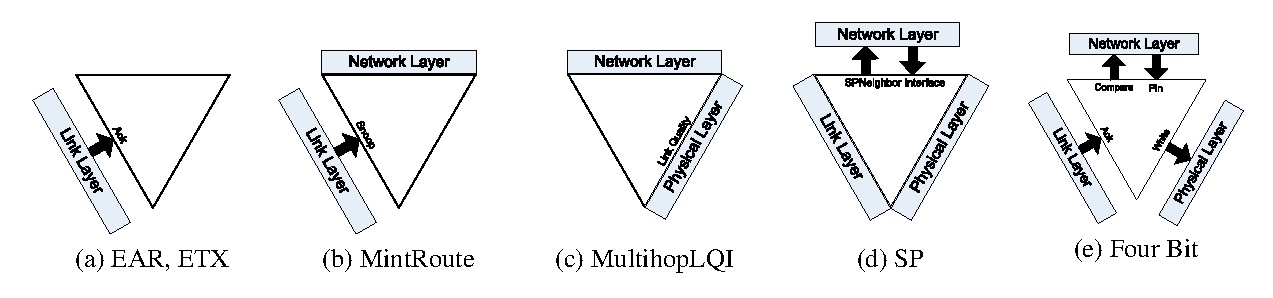
\includegraphics[scale=0.7]{figures/fig1}
\caption{每个图中间的三角形代表链路估计器与三个层间的相互联系。边上附着的框表示相结合的实现。指出的箭头表示估计器向接收到的包请求信息。指入的箭头表示某一层主动提供的信息。}\label{fig1}
\end{figure}

为了给我们的讨论打下基础,我们先看一种名为{\kai 汇聚}的多跳通信,多个节点用任意播的方式将数据发送到若干基站中的一个。这是在无线传感器网络中最常见的通信形式。然而我们的结论也同样适用与多数any-to-any多跳通信。

作为我们如何利用信息来作链路估计例子,我们先看TinyOS 2中的两种汇聚协议,汇聚树协议(CTP)\ucite{tep123}和MultiHopLQI\ucite{multihoplqi}。CTP使用基于检测的链路估计器,而MultiHotLQI仅依赖于CC2420无线芯片提供的链路质量指示器(LQI)。我们在有85个节点的测试平台上用较低的传输率作汇聚实验,每个节点隔10秒种产生一个包。图\ref{fig2}展示了CTP(a),MultiHopLQI(b),没有路由表大小限制的CTP(c)产生的路由树。同时它也标出了平均代价,即每个投递到的包的传输次数。较低的代价意味着较短的路径和较好的质量。

\begin{figure}[ht]
\centering
\subfigure[CTP(开销=3.14)]{
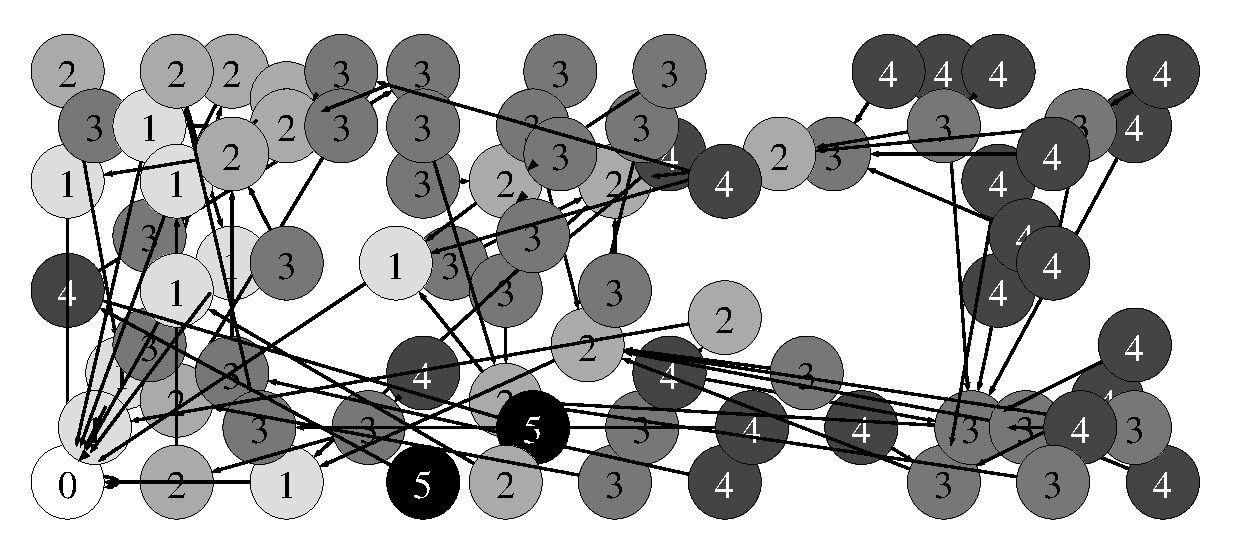
\includegraphics[scale=0.22]{figures/fig2a}}
\subfigure[MultiHopLQI(开销=2.28)]{
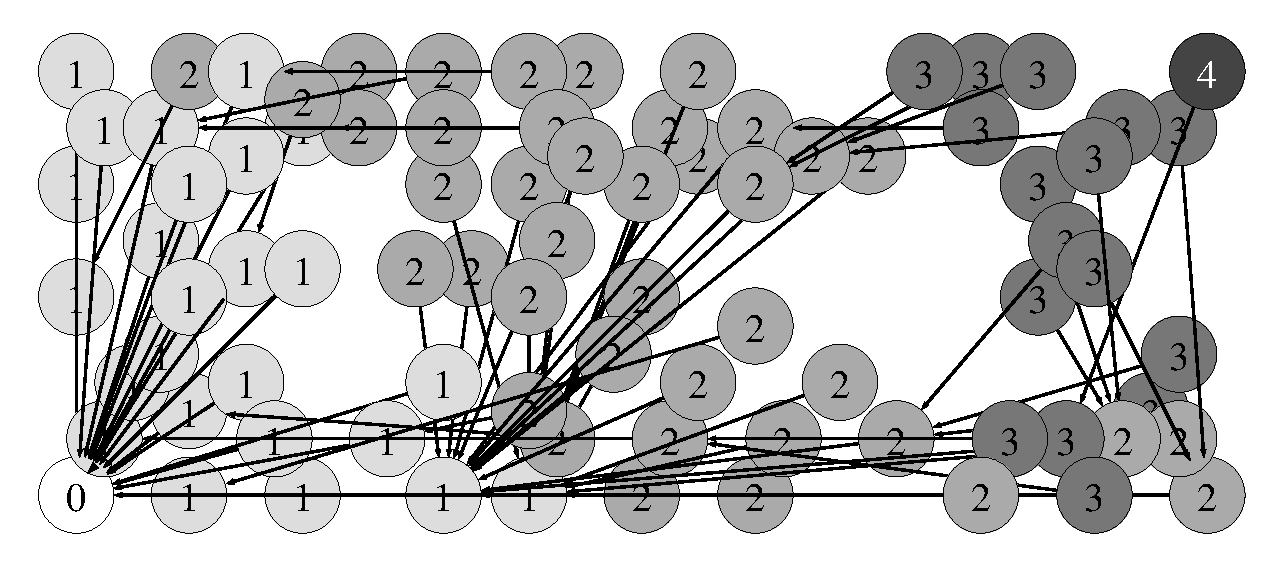
\includegraphics[scale=0.22]{figures/fig2b}}
\subfigure[不受限的CTP(开销=1.86)]{
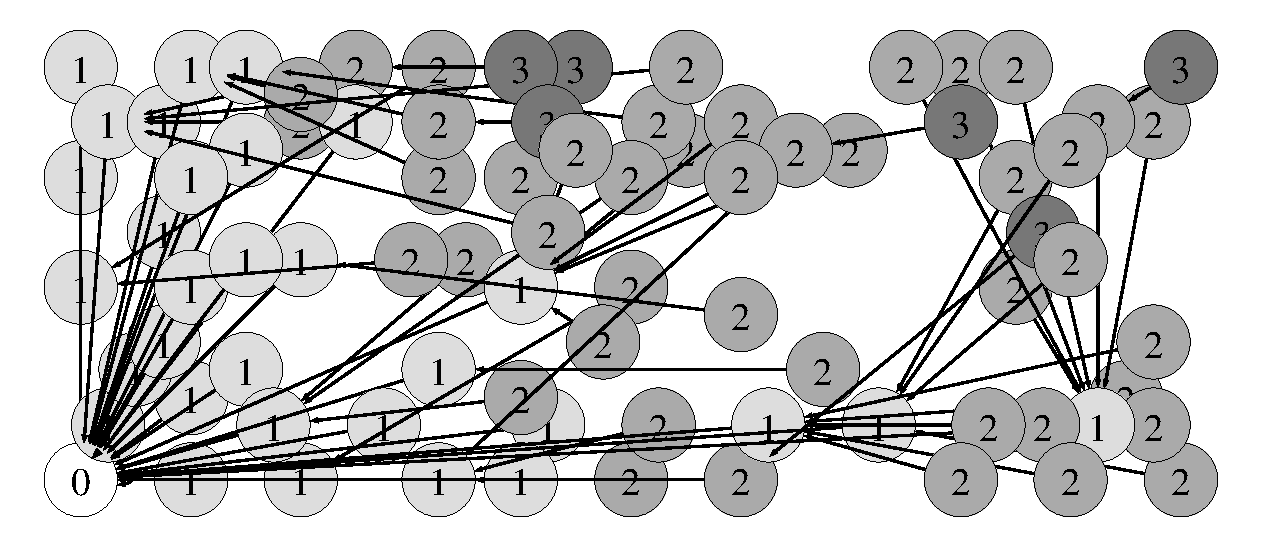
\includegraphics[scale=0.22]{figures/fig2c}}
\caption{由具有10个节点的连接表的CTP、MultiHopLQI和连接表不受限的CTP在85个节点上形成的路由树。在括号中指出了投递每个消息的平均开销。左下角的是根节点,颜色越暗的节点意味着到根的路径越长。}\label{fig2}
\end{figure}

CTP的开销比MultiHopLqi高,尽管后者只用到物理层的信息。这有两个原因:一是由于CTP使用双向的基于探测的链路估计器,它的连接表大小限制了节点的入度。第二,仍然是因为连接表的大小限制,它可能使最好的连接并不在连接表中。图\ref{fig2}展示了当连接表没有限制时,CTP胜过了MultiHopLQI。在第4节中,我们展示了如何使用物理层、链路层和网络层的信息来缓和这些问题。下面的小节详尽地讲述各层的利用价值和限制。

\subsection{物理层}
物理层可以通过解包来提供介质的质量信息。这个信息提供了一种避免边界或边缘问题的快速且廉价的方法。它可以增加估计器的灵敏度,并且为连接表项提供第一层过滤。在图\ref{fig2}中,MultiHopLQI(c)和SP(d)在链路估计中使用了物理层信息。

由于物理层信息属于单个包,并且它只能对收到的包作估计,故信道的变化会使它不准确。比如,在低功耗无线个人网络中,大多数连接是双向模式的\ucite{srinivasan2006ucp},在高质量(100\%PRR,packet reception ratio)和低质量(0\%PRR)间变化。在这种连接中,接收者如果只使用物理层的信息的话,那它将会发现许多高信道质量的包,从而认为该连接是好的,即使中间丢了不少包。

图\ref{fig3}展示了物理层信息的限制,我们观察了在94个节点上使用MultiHopLQI协议的12个小时低速率汇聚实验。如图\ref{fig1}所示,MultiHopLQI不使用链路层的信息。尽管总体上来看这个协议表现的不错,但是仍然有突发的包丢失现象。

\begin{figure}[ht]
\centering
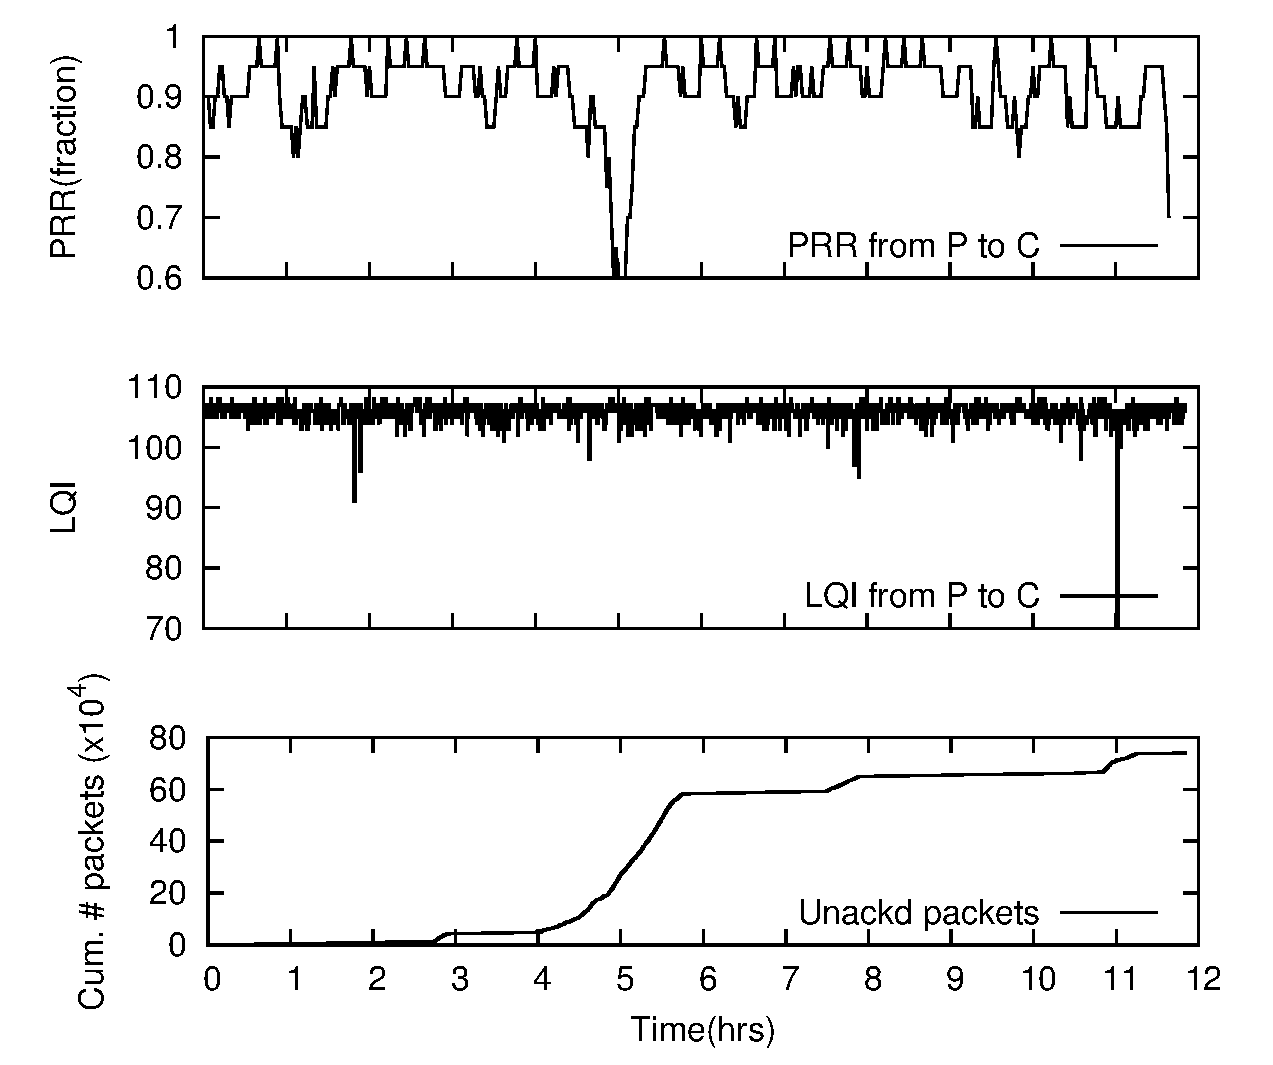
\includegraphics[scale=0.5]{figures/fig3}
\caption{由于没有意识到PRR的下降,MultiHopLQI在第4和第6个小时间尝试在同一条链路上发包从而导致由于重传而未被确认的包增加。}\label{fig3}
\end{figure}

如图\ref{fig3}所示,在一段时间中,节点C和P间的PRR从0.9降到将近0.6。这个连接质量的下降并不伴随着LQI解码质量的下降。C收到的包的质量都很好,但它并没有收到全部的包。

\subsection{链路层}

链路估计器如ETX和MintRoute使用周期性的广播来估计包的接收速率。这些估计器计算双向链路质量──包被传输并收到ACK的概率──即两个方向链路质量的乘积。虽然简单,这种方法适应地比较慢,并且需要假设周期性的广播和数据通信的行为相似。

通过使用2层的ACK统计收到ACK或没有收到ACK的包个数,链路估计器可以在同等的数据通信量上计算出更准确的估计值。这些估计值也是双向的。在图\ref{fig1}(a)中,EAR和ETX使用链路层的反馈来作链路估计。通过数据通信的链路层信息可以计算出比取控制包接收速率的乘积这种方式更精确的ETX。然而,尽管这很精确、很相关、很快速,但是发送数据包需要路由信息,而生成路由信息又需要链路质量估计值。这种自举最好在低层完成。同时,特别是在密集的网络中,选择合适的连接的集合来估计与如何计算估计值是同样重要的,如果仅在链路层做的话代价会比较昂贵。

\subsection{网络层}

物理层可以提供连接质量的粗略估计,让估计器避免在边缘或坏的连接上白花力气。一旦估计器估计了一个连接,网络层就可以决定哪些连接是有价值的。这在连接表有限的情况下是很重要的。比如,地域路由\ucite{karp2000ggp}可以从邻居是向各个方向平等的蔓延这一特性中获取有用信息,S4路由\ucite{mao2007sss}能从到信标的距离最小这一特性中获取有用信息。最近有一个不知名的无线传感器网络只能投递收集到的数据中的2\%,部分原因是由于网络层和链路层使用连接的不一致所造成。由于一些原因,MintRoute协议(图\ref{fig1}(b))在网络层中整合了链路估计器。SP(图\ref{fig1}(d))为网络层提供了丰富的接口,用于检查和更改估计器的邻居表。网络层发现邻居并作链路估计,但并不使用重传、ACK或是包解码质量这些信息,这样的估计是适应得较慢并且是代价昂贵的。

在下面的部分中我们描述了链路估计器如何有效地使用三层的信息,它只用4位的信息,而且有一些定义地很明确的接口。我们在第4节中演示了通过层间有效信息的交换使我们的接口的性能得到了很大的提升。

\section{设计}

第2部分展示了每层可以得到的有助于链路估计的信息。物理层可以为到达的包估计传输介质的质量。链路层可以知道包是否被传输并确认。网络层可以确定估计哪个连接是最值得的。本节提出了三层间的接口并描述了一个使用这些接口的链路估计器。

\subsection{估计接口}

图\ref{fig4}展示了各层为链路估计器提供的接口。三层总共提供4位的信息:两位用于到达的包,一位已传输的单播包,一位用于链路表项。

\begin{figure}[ht]
\centering
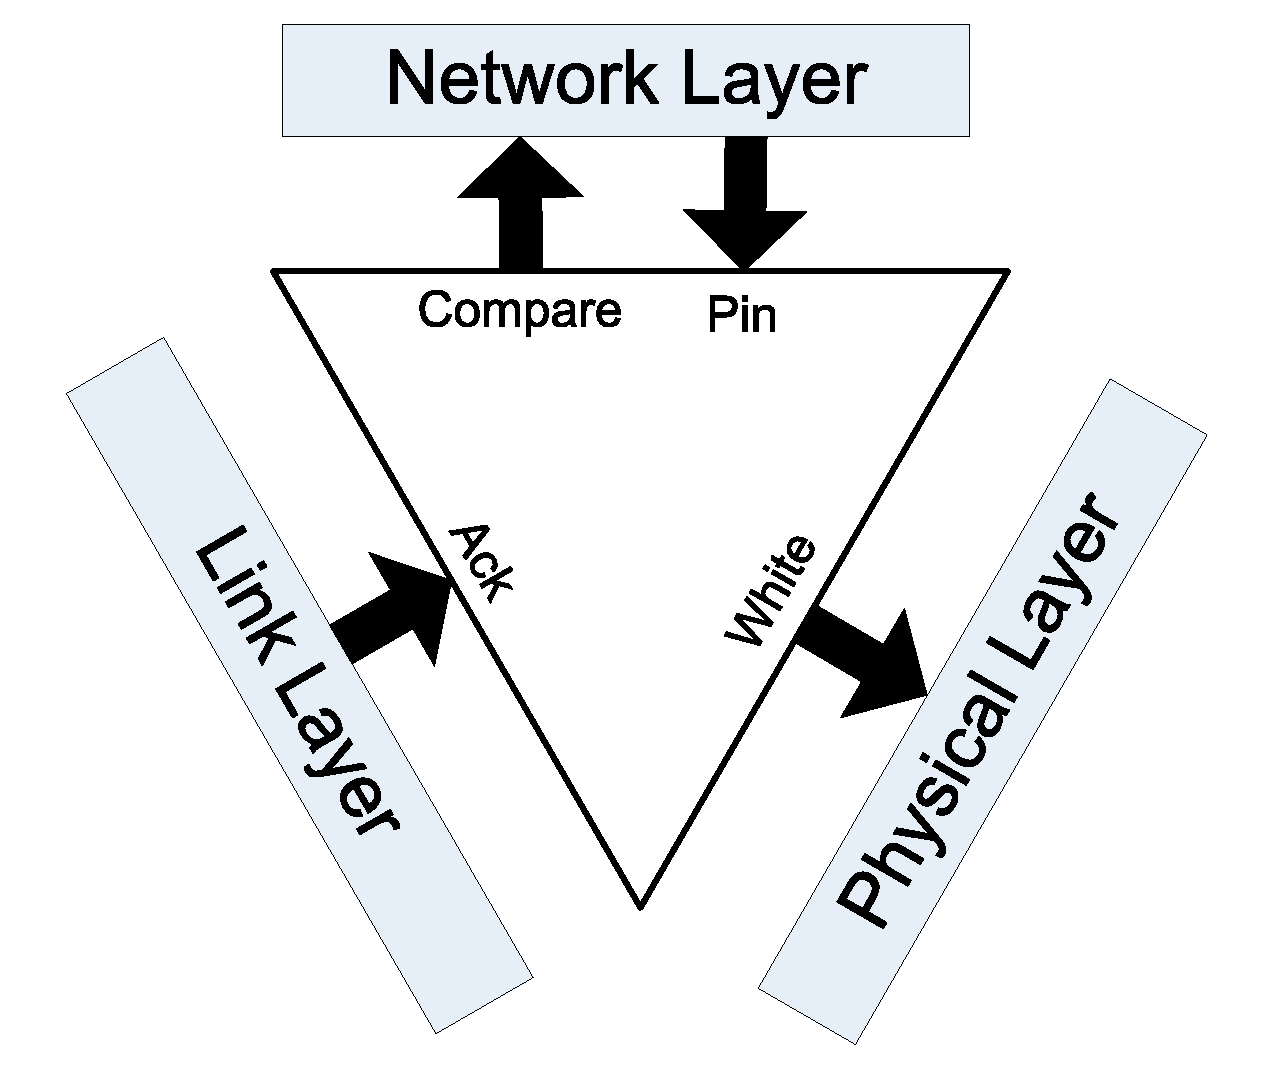
\includegraphics[scale=0.3]{figures/fig4}\label{fig4}
\caption{中间的三角形代表链路估计器,使用三个层的四位信息。指出的箭头表示估计器向接收到的包发出请求。指入的箭头表示某一层主动提供的信息。}
\end{figure}

物理层提供一位的信息。white位如果设为1,则表示接收到的包解码出错的概率很低。white位说明在接收中介质质量是很好的。反过来说则不一定正确。如果white位是0,则介质质量可能是不好的,也可能是好的。

链路层为每个已传输的包提供了一位的信息:ACK位。链路层在收到2层确认的时候设置ACK位。如果ACK位是0,则说明包可能没有成功地传输,也可能已经成功的传输了。

网络层提供了两位的信息,pin位和compare位。pin位用于连接表项。如果网络层在表项上设置了pin位,则链路估计器在pin位被清0前不能把它从表中移除。链路估计器可以为一个包向网络层获取compare位信息。compare位表示发送者提供的路由是否比连接表中的一项或多项要好。我们在3.3节中描述了链路估计器是如何使用compare位的。

\subsection{接口考虑}

我们认为4位的信息是链路估计器所需的信息的最小集合。此外,我们相信接口也足够简单,可以在大多数系统上实现。比如,无线的物理层提供的信号强度和噪声信号可以用于计算信噪比,根据信噪比错误率曲线,使用阀值的方法计算white位。物理层还可以使用比特错误恢复报告或芯片纠错率。在最坏的情况下,可以永不设置white位。

接口对链路层有一个限制:要有2层的同步确认。虽然这看上去要求很高,但其实大多数常用的链路层比如802.11和802.15.4都有这一功能。在这个模型中,新的或特定程序的链路层必须有2层确认。

compare位需要网络层能分辨包发送者的路由是否比连接表中的当前表项的路由要好。compare位并不要求网络层对所有的包都作比较,而只选择它们的一个子集。这意味着诸如路由信标中中会含有路由质量信息。

\subsection{一个混合的估计器}

我们将描述一个混合的估计器,它使用了周期性的信标帧,结合了三层的信息,提供精确、时效和有用的链路估计值。该估计器维护一个较小的连接表(比如大小为10),内含候选连接的ETX值。它周期性地广播含用这些连接信息的信标帧。网络层协议也通过估计器广播包,从而使它看起来像一个2.5层的协议,它在3层到2层的包中加头部加尾部。

估计器使用由Woo at al.\ucite{woo2003tuc}描述的表管理算法,但有一个例外:它并不假设最小传输率,因为它可以根据出站数据传输率来检测坏的连接。链路估计广播的包中含有顺序号,接收者使用它来计算信标接收率。

估计器使用white位和compare位对标准的表替换策略作补充。当它接收到一个white位为1的网络层的路由包并且发送者并不在连接表中时,估计器询问网络层compare位是否已设置。如果设置了,则估计器随机地剔除一个没有pin住的表项,并用当前包的发送者代替。

估计器使用ACK位使链路估计值更准确。结合广播和单播ETX估计为一个混合的值,这是一种在连接通信量不断变化的网络中使用的方法\ucite{kim2006aml}。我们使用Woo et al.\ucite{woo2003tuc}描述的链路估计方法,分别为单播包和广播包计算$k_u$或$k_b$个包的ETX值。如果$k_u$个发出的包中有$a$个被接收者确认,则单播包的ETX估计值为$\frac{k_u}{a}$。如果$a=0$,则估计值是从上次成功的接收算起的失败传输次数。对于广播包的估计也是类似的,但是有一个额外的步骤。我们在计算出的{\kai 接收率}上使用窗口化的指数移动平均值(EWMA),并转化连续的采样值为ETX值。从两种估计方法中得到的ETX值通过第二次EWMA结合起来,如图\ref{fig5}所示。结果是数据和信标窗口化EWMA估计值的混合。当数据流较大时,单播包的估计值占主导地位。当网络比较安静时,广播估计占主导地位。

\begin{figure}[ht]
\centering
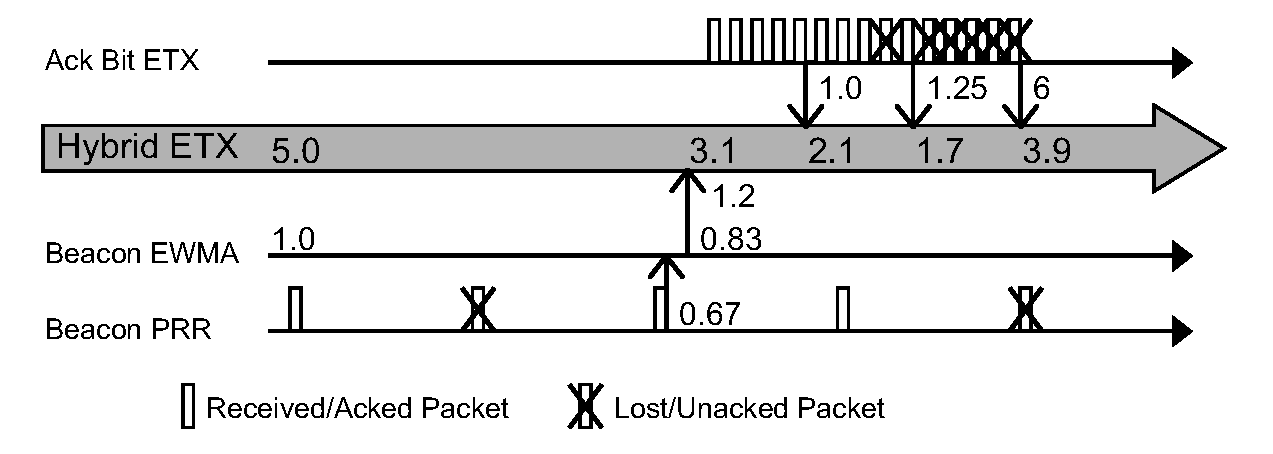
\includegraphics[scale=0.5]{figures/fig5}\label{fig5}
\caption{我们的链路估计器结合了单播包和广播通信的估计生成ETX值,使用的窗口大小分别为$k_u=5$和$k_b=2$。后者在结合之前要对自身作一次平均。我们用小方框表示到来的包,给丢失的包标上“$\times$”。估计器在垂直箭头处计算估计值。}
\end{figure}

与大多数纯广播的估计器相比,我们的估计器并不通过信标帧积极地交换和维护双向估计值。因为ack位也可以测量双向连接特性,因而我们的估计器可以避免只使用信标帧估计作为链路估计的自举值。这是一个很重要的特性,它把网络拓扑中的节点入度从连接表中分离出来。

\section{评价}

我们在TinyOS 2中实现了3.3节所描述的链路估计器原型,通过替换CTP中标准的链路估计器来测试它。我们的估计器对物理层、链路层、网络层使用4位接口,我们修改了CTP中的这些层以使用该接口。在本节中,我们通过实验和比较详细地评测了我们的原型、原来的CTP和MultiHopLQI。在下面的讨论中,我们的原型称为“4B”。MultihopLQI如上面所述所用了链路质量指示器(LQI),这是CC2420无线模块具有的特性,对具有该模块的系统来说,MultihopLQI是目前TinyOS中性能最好的汇聚协议实现。

在比较中,我们在Mirage测试平台上运行了这三个协议,用85个MicaZ节点,其中一个节点作为基站。同时我们也在另一个测试平台TutorNet上作了测试,使用了94个TelosB节点。传输功率若非特别指出都设为0dBm。在每个实验中,我们使用统一分布错开启动时间在30秒的范围内。每个节点发送一个有些许抖动的汇聚包以避免与其它包产生包同步。每个节点提供的工作负载是常数速率发送到根节点的包流。这会使网络中产生并发的传输流汇聚到根节点。在Mirage上实验时间在40到60分钟之间。在TutorNet上的实验时间则要长的多,在3到12小时左右。测试平台是静态的并且我们所有的实验结果在各个实验平台上一致,这给了我们信心确信较短的运行时间得出的结果也将是一致的。

我们评价性能的主要标准是{\kai 开销}:每个单播包传输的总次数。开销的重要性在于它直接联系到网络的生存时间。它考虑了路径的跳数、每个连接的重传数以及由于包丢失而造成的浪费。为了考虑开销,我们也注意到了拓扑树的平均深度。如果所有的连接是完好的,平均深度将是开销的下界。两者间的差异意味着选择连接的质量,这可能是由于重传或丢包所造成的。最后我们还考查了投递率,即根节点收到唯一消息的百分率。

我们首先看3.1节中附加的每个位是如何影响开销和路由长度的。我们比较原来的CTP和4B,以及两种中间的实现。在图\ref{fig6}中左边最上面的点展示了运行在Mirage测试平台上的CTP的开销和深度。为CTP增加单向链路估计和ack位能减少93\%的平均树深度,并减少31\%的开销。单向估计把入度从连接表大小中分离出来,因此深度大大减小。

\begin{figure}[ht]
\centering
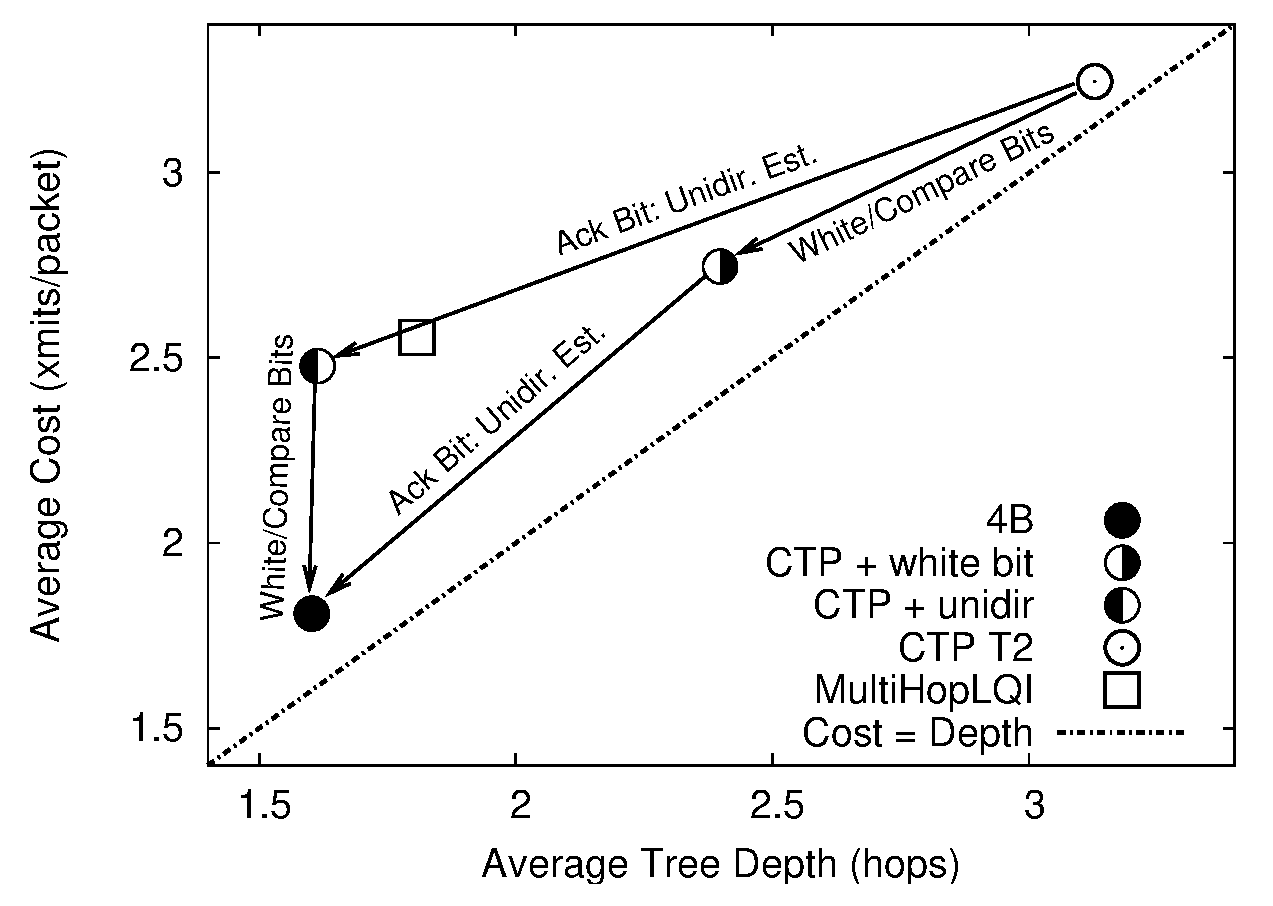
\includegraphics[scale=0.5]{figures/fig6}\label{fig6}
\caption{在CTP中增加ack位、white位和compare位以降低开销(越低越好)和节点在路由树中平均深度。}
\end{figure}

与原来的CTP相比,增加white和compare位能减少55\%的开销,这可能是因为父结点的选择得到了改进。为CTP仅增加white和compare位使开销减少15\%,平均深度减少23\%。该图还列出了在相同测试平台上的MultiHopLQI的开销和深度以作比较。仅当我们使用全部三层的信息时,4B才比MultiHopLQI好。4B的开销要低29\%,路径要短11\%。在TutorNet测度平台上,4B的开销和平均深度相应的比MultiHopLQI低44\%和9.7\%。4B产生的树和平均树深度与不限制路由表大小的CTP(图2)非常类似。

图\ref{fig7}比较了在Mirage测试平台上的4B和MultihopLQI的开销和平均节点深度。发射功率在-20dBm到0dBm间变化。在每个协议中,我们看到平均节点深度和开销随着传输功率的减小而增大,因为节点需要经过更多跳的路由。4B相对于MultihopLQI在开销方面的改进在11\%到29\%之间,而在平均深度上的改进在11\%到3.5\%之间。在0到-10dBm间,4B的开销最多也就是下界的13\%,而MutiHopLQI的是43.4\%。在多跳网络中,这两个协议都效果不好,相应开销的增加(平均深度4B增加62\%以上,MultiHopLQI为95\%)意味着重传和包丢失增加。即使树深度相似,4B能选择更好的连接。

\begin{figure}[ht]
\centering
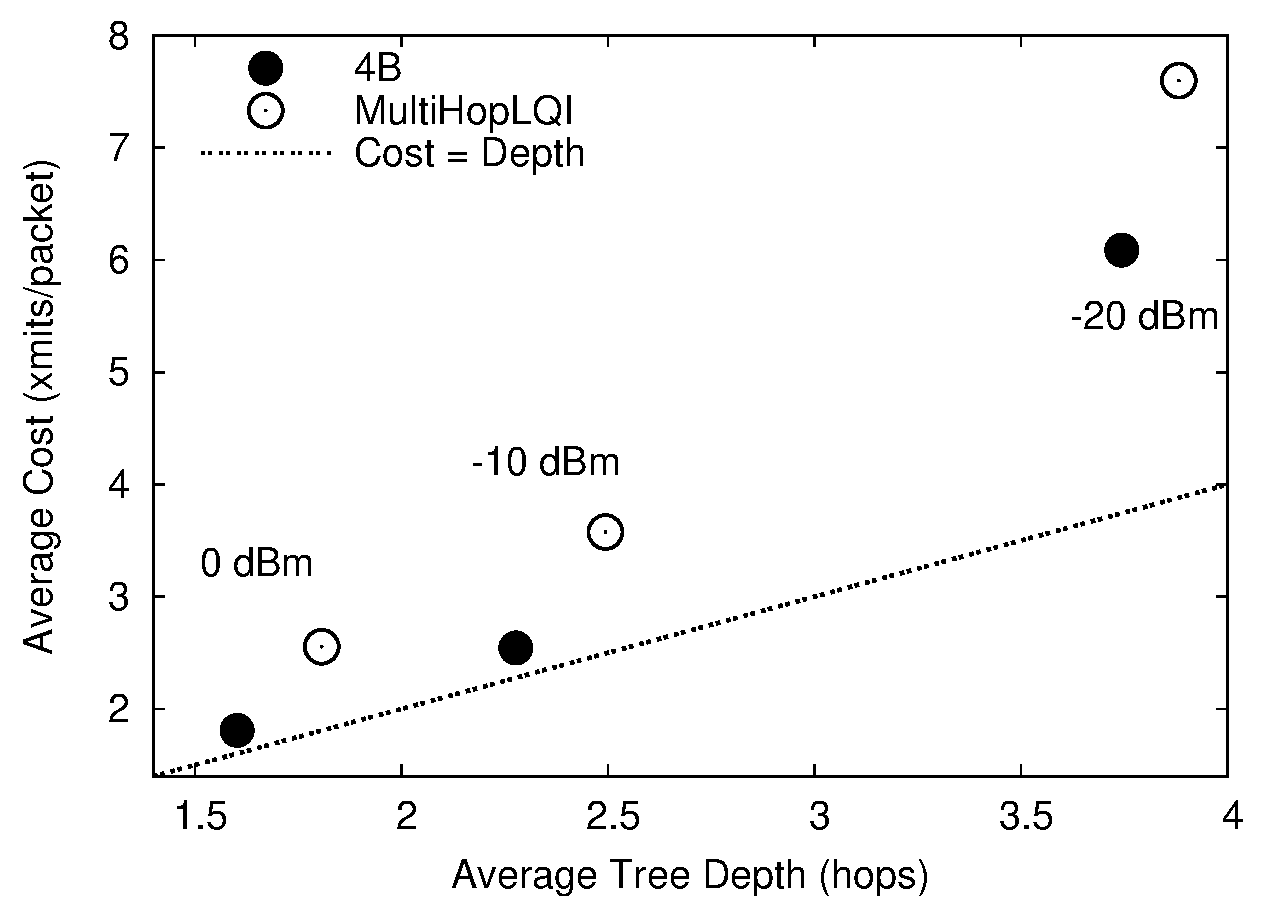
\includegraphics[scale=0.5]{figures/fig7}\label{fig7}
\caption{在Mirage测试平台上降低传输功率时MultiHopLQI和4B的平均节点深度和开销。4B可以降低19\%-28\%的开销。}
\end{figure}


图\ref{fig8}展示了每个节点的投递率,并解释了图\ref{fig4}中开销比平均树深度增长地快的原因。在0到10dBm间,4B的平均投递率在99.9\%以上,最低是99.3\%。在0dBm时,MultihopLQI的平均投递率为是95.9\%,最坏的节点是64\%。当发射功率下降时,相应的RF噪声的影响加重,使网络中局部不对称。如第2节中的例子,MultihopLQI的性能下降是由于这种连接质量的变化不能被物理层指示器捕捉到。我们打算观察网络的动态行为,但是即使在-20dBm下,4B的包丢失数也很少,这意味着开销的增大主要由于重传,而不是包丢失。这说明估计器足够灵敏,可以检测到包丢失并切换到新的路由。

\begin{figure}[ht]
\centering
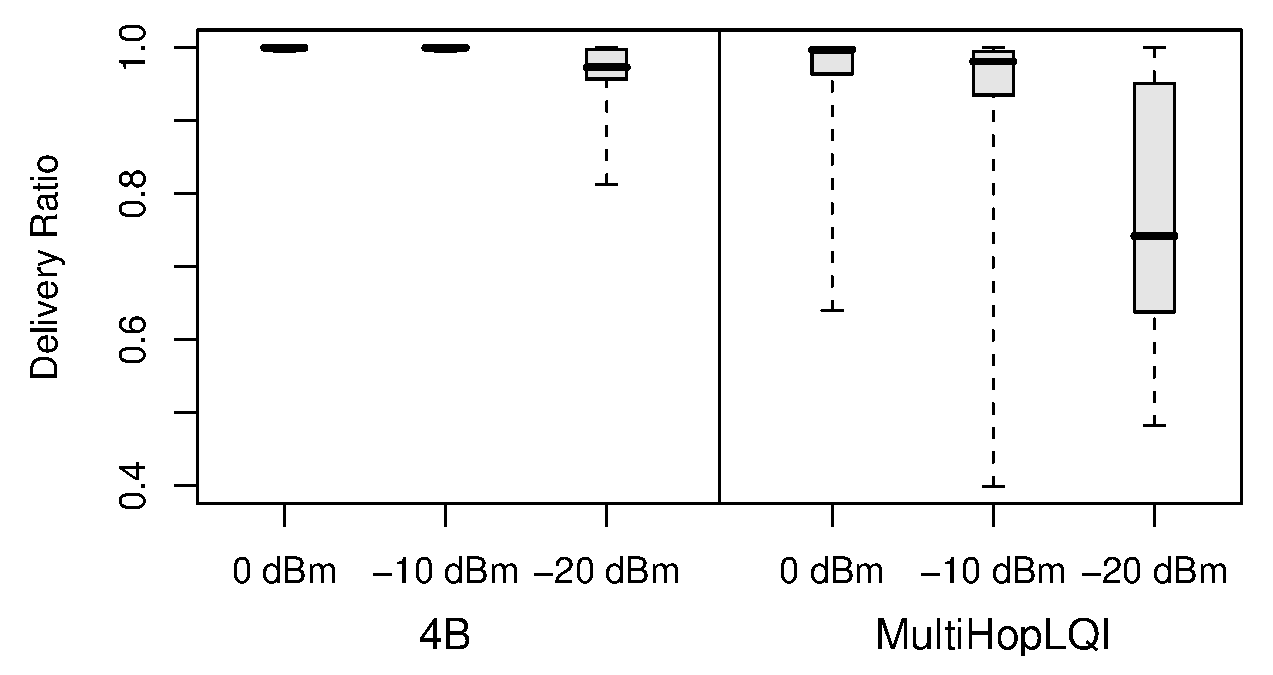
\includegraphics[scale=0.5]{figures/fig8}\label{fig8}
\caption{在发送功率逐渐降低的情况下,4B和MultihopLQI中每个节点的投递率分布框图。端点表示最大和最小值。框表示四分之一和四分之三的位置。粗线是中位线。4B维持了较高和较一致的投递率。}
\end{figure}

\section{结论}

在本文中我们提出了一个窄的、完善定义的接口,它允许链路估计器使用来自物理层、链路层和网络层的信息。我们的原型展示了在开销和投递率上很大的改进,同时也保持了网络的分层抽象结构。这是令人鼓舞的,因为我们还没有完全掌握使用4位接口的所有特性。一个可移植、精确和有效的链路估计器在规模与日俱增的网络、低功耗的IP扩展和像IETF 6lowpan这类嵌入式网络中越来越重要。比如,TCP的性能是对包丢失非常敏感的,通过使用我们的链路估计器达到的改进可能会对端到端的吞吐量产生很大的影响。

\wuhao
\bibliographystyle{plain}
\bibliography{reference/reference}

\end{document}
